\documentclass[14pt]{beamer}

\mode<presentation> {
\usetheme{Madrid}

% To remove the navigation symbols from the bottom of all slides uncomment next line
\setbeamertemplate{navigation symbols}{} 
\date{}
\title{}
\author{}

%to get rid of footer entirely uncomment next line
\setbeamertemplate{footline}{}
}


\usepackage{geometry}
\usepackage{multirow}
\usepackage{adjustbox}
\usepackage{multicol}
\setlength{\columnsep}{0.1cm}



\usepackage{tikz}
\usetikzlibrary{shapes,backgrounds}

\usepackage{bbding}
\usepackage{rotating}
\usepackage{xcolor}


%\usepackage{tkz-berge} %cool grid
\usepackage{pgfplots} %pics

\usepackage{graphicx} % Allows including images
\usepackage{booktabs} % Allows the use of \toprule, \midrule and \bottomrule in tables
\usepackage{mathtools}

\newcommand {\DS} [1] {${\displaystyle #1}$}
\newcommand {\R}{\mathbb{R}}
\newcommand {\Z}{\mathbb{Z}}
\newcommand {\N}{\mathbb{N}}
\newcommand{\e}{\varepsilon}

\newcommand{\p}{\pause}

% simple environrment for enumerate, easier to read
\setbeamertemplate{enumerate items}[default]

%%%%%%%%%%%%%%%%%%%%%%

% to use colours easily
\definecolor{miverde}{rgb}{0.7, .5, 0.7}
\newcommand{\azul}[1]{{\color{blue} #1}}
\newcommand{\rojo}[1]{{\color{red} #1}}
\newcommand{\verde}[1]{{\color{miverde} #1}}
 
% box in red and blue in math and outside of math
\newcommand{\cajar}[1]{\boxed{\mbox{\rojo{ #1}}}}
\newcommand{\majar}[1]{\boxed{\rojo{ #1}}}
\newcommand{\cajab}[1]{\boxed{\mbox{\azul{ #1}}}}
\newcommand{\majab}[1]{\boxed{\azul{ #1}}}
 
\newcommand{\setsize}[1]{\fontsize{#1}{#1}\selectfont} %allows you to change the font size. The default size of this document is 14. To change the font size of the whole slide, place this at the beginning of the slide. To change the size of only a portion of the text to size 12, you can do the following { \setsize{12} Your text. }.

\setbeamerfont{frametitle}{size=\setsize{15}}
\setbeamerfont{block title}{size=\setsize{14}}

\newcommand{\smallerfont}{\setsize{13}} %place this at the beginning of a slide to set the font size of the entire slide to 13.


\setbeamertemplate{enumerate items}{(\Alph{enumi})}


%===========================

%===================================================
\begin{document}
%===================================================


\begin{frame}
	\frametitle{MAT137 Lecture 17 --- Definition of Derivative}

	\vfill
	{\bf Before next class:}
		\begin{itemize} \normalsize
			\item {\bf Watch videos 3.4, 3.5, 3.8 }
		\end{itemize}
\end{frame}


%-----------------------------
\begin{frame}[t]
\frametitle{Tangent line to a line?}

What is the equation of the line tangent to the graph of $y=x$ at the point with $x$--coordinate $7$?

\
\begin{enumerate}
	\item \DS{y=x+7}
	\item   \DS{y=x}
	\item  \DS{y=7}
	\item  \DS{x=7}
	\item  There is no tangent line at that point.
	\item  There is more than one tangent line at that point.
\end{enumerate}

\end{frame}
%-----------------------------

\begin{frame}
\frametitle{Prove these statements are false with counterexamples}

Let  $C$ be a curve. 
Let $P$ be a point in $C$.
\vfill
\begin{enumerate}
	\item The line tangent to $C$ at $P$ \\ intersects $C$ at only one point: $P$.
\vfill
	\item  If a line intersects $C$ only at $P$, \\ then that line must be the tangent line to $C$ at $P$.
\vfill
	\item  The tangent line to $C$ at $P$ intersects $C$ at $P$ \\ and ``does not cross'' $C$ at $P$.  \\ (This means that, near $P$, it stays on one side of $C$.)
\vfill
	\item  If a line intersects $C$ at $P$ \\ and ``does not cross'' $C$ at $P$, \\ then it is the tangent line to $C$ at $P$.
\vfill
\end{enumerate}

\end{frame}

%-----------------------------
\begin{frame}[t]
\frametitle{Tangent line from a graph}
	This is the graph of the function $f$.  Write the (approximate)
	equation of the line tangent to it at the point with $x$--coordinate $-2$.
\begin{center}
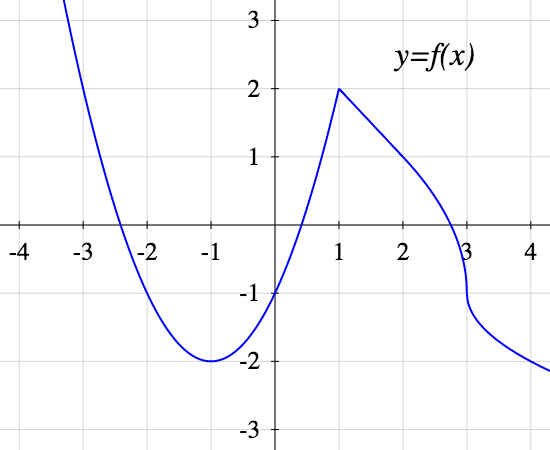
\includegraphics[scale=.4]{G4}
\end{center}

\end{frame}
\begin{frame}[t]
\frametitle{Tangent line from a graph}
	This is the graph of the function $f$.  Write the (approximate)
	equation of the line tangent to it at the point with $x$--coordinate $-1$.
\begin{center}
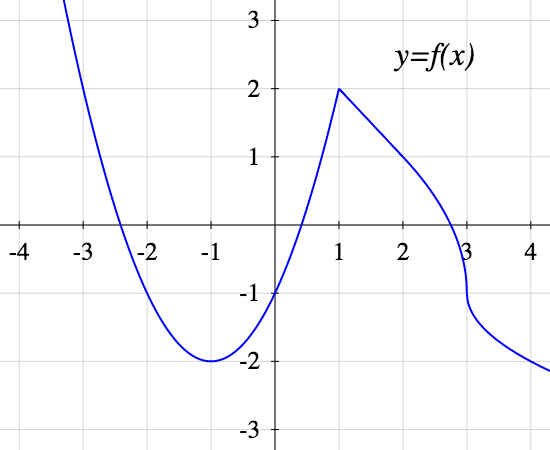
\includegraphics[scale=.4]{G4}
\end{center}

\end{frame}
%-----------------------------
\begin{frame}[t]
\frametitle{Derivative from a graph}
This is the graph of the function $f$.  \\
Sketch the graph of its derivative $f'$.
\begin{center}
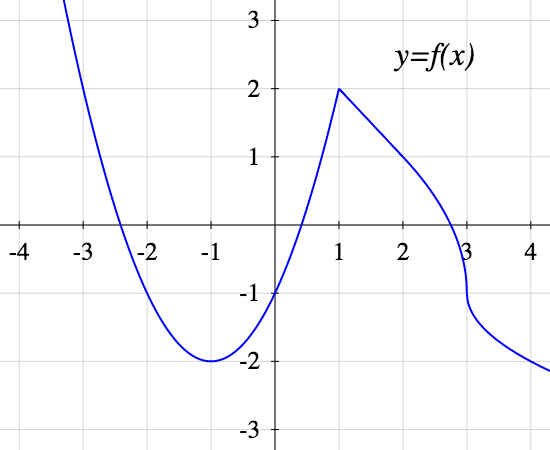
\includegraphics[scale=.4]{G4}
\end{center}

\end{frame}
\begin{frame}[t]
\frametitle{Derivatives from the definition}

Let 
	$$g(x) = \frac{2}{\sqrt{x}} $$
	
Calculate \DS{g'(4)} directly from the definition of derivative as a limit.

\end{frame}

%-----------------------------



\begin{frame}
	\frametitle{MAT137 Lecture 18 --- Differentiation Rules}

	{\bf Warmup:}

	Sketch $y=f'(x)$.

\begin{center}
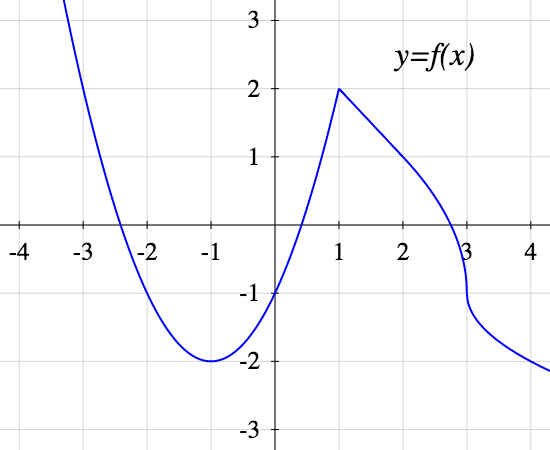
\includegraphics[scale=.3]{G4}
\end{center}
	\vfill
	{\bf Before next class:}
		\begin{itemize} \normalsize
			\item {\bf Watch videos 3.6, 3.7, 3.9 }
		\end{itemize}
\end{frame}

\begin{frame}[t]
\frametitle{Differentiable functions}

Let $a \in \R$.  \\
Let $f$ be a function with domain $\R$.  \\
Assume $f$ is differentiable everywhere.  \\
What can we conclude?

\begin{multicols}{2}
\begin{enumerate}
	\item  $f(a)$ is defined.
	\item \DS{\lim_{x \to a} f(x)} exists.
	\item  $f$ is continuous at $a$.
	\item  $f'(a)$ exists.
	\item  \DS{\lim_{x \to a} f'(x)} exists.
	\item  \DS{f'} is continuous at $a$.
\end{enumerate}
\end{multicols}
 
\end{frame}

\begin{frame}
\frametitle{Computations: Basic differentiation rules}

Compute the derivative of the following functions:

\
\begin{multicols}{2}
\begin{enumerate}
	\item  \DS{f(x) = x^{100} - 3x^{9} - 2}

\

	\item  \DS{f(x) = \sqrt[3]{x} + 6}

\

	\item  \DS{f(x) = \frac{4}{x^4}}

\

	\item  \DS{f(x) = \sqrt{x} \left( 1 + 2x \right)}

\

	\item  \DS{f(x) = \frac{x^6+ 1}{x^3}}

\

	\item  \DS{f(x) = \frac{x^2-2}{x^2+2}}
\end{enumerate}
\end{multicols}

\end{frame}

\begin{frame}[t]
\frametitle{Higher order derivatives}


Let \DS{g(x) = \frac{1}{x^3}}.

\

\begin{itemize}
	\item Calculate the first few derivatives.  
	\item Make a conjecture for a formula for  the $n$-th derivative \DS{g^{(n)}(x)}.
	\item  Prove it by induction.
\end{itemize}

\end{frame}

%-----------------------------

\begin{frame}
\frametitle{Estimations -- 2}


Without using a calculator, estimate \DS{\sqrt[20]{1.01}} as well as you can.

\

\emph{Hint:}  You know the value of \DS{f(x) = \sqrt[20]{x}} and its derivative at one point very close to 1.01.  Use the tangent line at that point as an approximation.
 
\end{frame}
%-----------------------------
\begin{frame}[t]
\smallerfont
\frametitle{Estimations -- 3}

%The point of this question is to make them discover L'Hopital's Rule!


\begin{enumerate}
\item  We know \quad
	\DS{
		f(0) = 2, \quad f'(0) = 3, \quad g(0) = 7, \quad g'(0) = 5.
	}
	
	\vspace{.2cm}
 	Compute \; \DS{\lim_{x \to 0} \frac{f(x)}{g(x)}}.

\vfill

\item  We know \quad 
	\DS{
		f(0) = 0, \quad f'(0) = 3, \quad g(0) = 0, \quad g'(0) = 5.
	}
	
	\vspace{.2cm}
 	\begin{itemize}
		\item  When $x$ is close to $0$, give estimates for \DS{f(x)} and \DS{g(x)} using the tangent lines at $0$. 
		\item Use those estimates to compute \;  \DS{\lim_{x \to 0} \frac{f(x)}{g(x)}}.
	\end{itemize}
	
\end{enumerate}
 
 \vfill
 
\end{frame}




















\begin{frame}
	\frametitle{MAT137 Lecture 19 --- Proof of Differentiation Rules}

	\vfill
	{\bf Before next class:}
		\begin{itemize} \normalsize
			\item {\bf Watch videos 3.10, 3.11 }
		\end{itemize}
\end{frame}

\begin{frame}
\frametitle{Estimations - 1}

Let $f$ be a continuous function with domain $\R$.

\vfill

\begin{enumerate}
	\item  We know $f(4)=3$ and $f(4.2)=2.2$.  \\
		Based only on this, give your best estimate for $f(4.1)$.
\vfill

	\item  We know $f(4)=3$ and $f'(4)=0.6$. \\
		Based only on this, give your best estimate for $f(4.1)$.
\vfill
		
	\item  We know $f(4)=3$ and $f(4.1) = 4$. \\
		Based only on this, give your best estimate for $f'(4)$.	
\end{enumerate}

\vfill

\end{frame}


\begin{frame}[t]
\smallerfont
\frametitle{True or False - Differentiability vs Continuity}

Let $f$ be a function with domain $\R$.  Let $c \in \R$. \\
Which of these implications are true?

\vfill

\begin{enumerate}
	\item IF $f$ is \rojo{continuous} at $c$, THEN $f$ is \azul{differentiable} at $c$
\vfill
	\item IF $f$ is \azul{differentiable} at $c$, THEN $f$ is \rojo{continuous} at $c$
\vfill
	\item IF $f$ is \azul{differentiable} at $c$, THEN $f'$ is \rojo{continuous} at $c$
\vfill
	\item IF $f'$ is \rojo{continuous} at $c$, THEN $f$ is \rojo{continuous} at $c$
\vfill
	\item IF $f$ is \azul{differentiable} at $c$, THEN $f$ is \rojo{continuous} at and near $c$.
\vfill
	\item IF $f$ is \rojo{continuous} at and near $c$, THEN $f$ is \azul{differentiable} at $c$.
\vfill
\end{enumerate}
 
\end{frame}
%-----------------------------
\begin{frame}[t]
\smallerfont
\frametitle{True or False - Differentiability and Operations}

Let $f$ be a function with domain $\R$.  Let $c \in \R$. \\
Let \DS{g(x) = f(x)^2}.
Which of these implications are true?

\vfill

\begin{enumerate}
	\item IF $f$ is \azul{differentiable} at $c$, THEN $f+f'$ is \rojo{continuous} at $c$
\vfill
	\item IF $f$ is \azul{differentiable} at $c$, THEN $3f$ is \azul{differentiable} at $c$.
\vfill
	\item IF $f$ is \azul{differentiable} at $c$, THEN $g$ is \azul{differentiable} at $c$.
\vfill
	\item IF $g$ is \azul{differentiable} at $c$, THEN $f$ is \azul{differentiable} at $c$.
\vfill
	\item IF $f$ is \azul{differentiable} at $c$, THEN $1/f$ is \azul{differentiable} at $c$.
\vfill
\end{enumerate}
 
\end{frame}


\begin{frame}[t]
\frametitle{Absolute value and tangent lines}


At (0,0) the graph of \DS{y=|x|}...
	\begin{enumerate}
		\item ... has one tangent line: $y=0$
		\item ... has one tangent line: $x=0$
		\item ... has two tangent lines $y=x$ and $y=-x$
		\item ... has no tangent line
	\end{enumerate} 

\begin{center}
	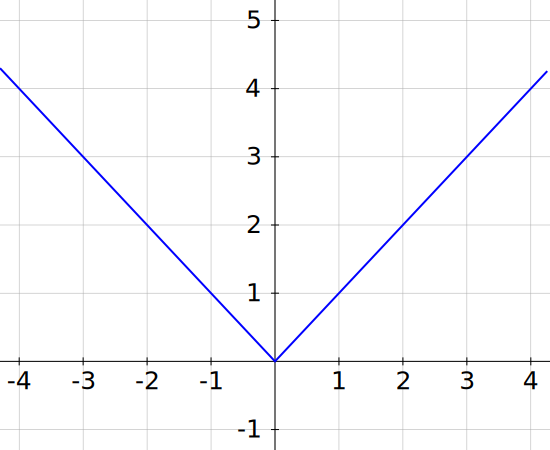
\includegraphics[scale=.25]{G8}
\end{center}

\end{frame}

%-----------------------------
\begin{frame}[t]
\frametitle{Absolute value and derivatives}

	Let $h(x) = x|x|$.  What is $h'(0)$?

\
\begin{enumerate}
	\item It is 0.
	\item It doesn't exist because $|x|$ is not differentiable at $0$.
	\item It doesn't exist because the right- and left-limits, when computing the derivative, are different.
	\item  It doesn't exist because it has a corner.
	\item It doesn't exist for a different reason.
\end{enumerate}


\end{frame}

\begin{frame}[t]
\smallerfont
\frametitle{Write a proof for the quotient rule for derivatives}

\begin{block}{Theorem}
\begin{itemize}
	\item Let $a \in \R$.
	\item  Let $f$ and $g$ be functions defined at and near $a$. \\
		Assume $g(x) \neq 0$ for $x$ close to $a$.
	\item  We define the function $h$ by  \DS{h(x) = \frac{f(x)}{g(x)}}.
\end{itemize}

IF $f$ and $g$ are differentiable at $a$, \\
THEN  $h$ is differentiable at $a$, and
	$$
		h'(a) =  \frac{f'(a) g(a) - f(a) g'(a)}{g(a)^2}.
	$$
\end{block}

\vfill


Write a proof directly from the definition of derivative.

\emph{Hint:} Imitate the proof of the product rule in  Video 3.6.

\end{frame}

%-----------------------------
\begin{frame}[t]
\frametitle{Check your proof}

\begin{enumerate}
	\item Did you use the \emph{definition} of derivative?
	\item  Are there words or only equations?
	\item  Does every step follow logically?
	\item  Did you only assume things you could assume?
	
	\
	
	\item  Did you assume at some point that a function was differentiable?  If so, did you justify it?

	\item \label{qu:cont} Did you assume at some point that a function was continuous?  If so, did you justify it?
	
\end{enumerate}

\

If you answered ``no" to Q\ref{qu:cont}, you probably missed something important.

\end{frame}
%-----------------------------
\begin{frame}[t]
\smallerfont
\frametitle{Critique this proof}
\vspace{-1cm}
	\begin{align*}
		h'(a) \; &= \;
			\lim_{x \to a} \frac{h(x) - h(a) }{x - a} \; = \; \lim_{x \to a} \frac{\; \dfrac{f(x)}{g(x)} \; - \; \dfrac{f(a)}{g(a)} \;}{x-a}
		\\ \ \\ & = \;
			\lim_{x \to a} \frac{f(x)g(a) - f(a)g(x)}{g(x)g(a) \; (x-a)}
			\\ \ \\& = \;
			\lim_{x \to a} \frac{f(x)g(a) - f(a)g(a) + f(a)g(a) - f(a) g(x)}{g(x) g(a) \; (x-a)}
			\\ \ \\ & = \;
			\lim_{x \to a} \left\{ \left[   \frac{f(x) - f(a)}{x-a} g(a) - f(a) \frac{g(x) - g(a)}{x-a} \right] \frac{1}{g(x) g(a)} \right\}
			\\ \ \\ & = \;
			\left[ f'(a) g(a) - f(a) g'(a) \right] \frac{1}{g(a) g(a)}
	\end{align*}
\end{frame}





















\begin{frame}
	\frametitle{MAT137 Lecture 20 --- The Chain Rule}

	\vfill
	{\bf Before next class:}
		\begin{itemize} \normalsize
			\item {\bf Watch videos 3.12, 3.13 }
		\end{itemize}
\end{frame}


\begin{frame}
\frametitle{Quick composition}

 Let $f$ and $g$ be differentiable functions and let $h=f\circ g$. \\ What is $h^{\prime}(2)$?
\begin {enumerate}
\item $f^{\prime}(2)\circ g^{\prime}(2)$
\item $f^{\prime}(2)g^{\prime}(2)$
\item $f^{\prime}(g(2)) g^{\prime}(2)$
\item $f^{\prime}(g(x)) g^{\prime}(2)$
\end{enumerate}

%Answer: (c). Even though students may have memorized the Chain Rule formula, some may not be able to apply it to this type of problem.
\end{frame}

%-----------------------------
\begin{frame}[t]
\frametitle{True or False - Differentiability and Composition}

Let $f$ and $g$ be functions with domain $\R$.  Let $c \in \R$. \\
Assume $f$ and $g$ are differentiable at $c$.  \\
What can we conclude?

\vfill

\begin{enumerate}
	
	\item $f \circ g$ \; is \azul{differentiable} at $c$.
\vfill
	\item $f \circ f$ \; is \azul{differentiable} at $c$.
\vfill
	\item $f \circ \sin$ \; is \azul{differentiable} at $c$.
\vfill
	\item $\sin \circ f$ \; is \azul{differentiable} at $c$.
\vfill
\end{enumerate}
 
\end{frame}
%-----------------------------

\begin{frame}[t]
\frametitle{Computations: Chain rule}

Compute the derivative of 

\

\begin{enumerate}
	\item  \DS{f(x) = \left( 2x^2+x+1 \right)^{8} }


\
	
	\item \DS{f(x) = \frac{1}{\left( x + \sqrt{x^2+x}  \right)^{137}}  }

\end{enumerate}

\end{frame}














\begin{frame}
	\frametitle{MAT137 Lecture 21 --- Trig Derivatives and Implicit Differentiation}

	\vfill
	{\bf Before next class:}
		\begin{itemize} \normalsize
			\item {\bf Watch videos 4.1, 4.2 }
		\end{itemize}
\end{frame}

















%----------------------------------------------------------------------------------------
%	DERIVATIVE AS SLOPE
%----------------------------------------------------------------------------------------

\begin{frame}[t]
\frametitle{From the derivative to the function}

\begin{enumerate}
	\item Sketch the graph of a continuous function with domain $\R$, whose derivative has the graph below.
	\item Sketch the graph of a non-continuous function whose derivative has the graph below.
\end{enumerate}

\begin{center}
	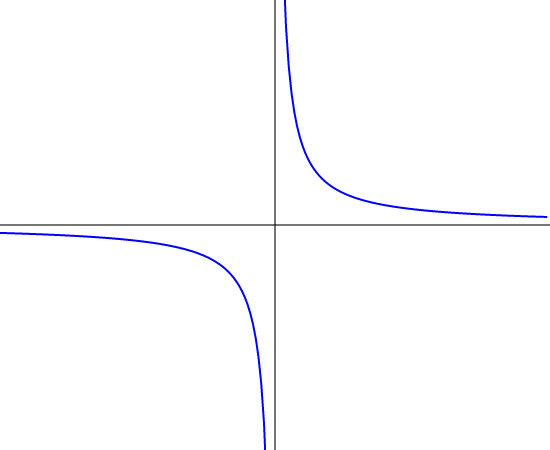
\includegraphics[scale=.3]{G5}
\end{center}

\end{frame}

%-----------------------------


%-----------------------------
%  Derivative from the definition
%-----------------------------
%-----------------------------

%-----------------------------
% Derivative as rate of change
%-----------------------------
%-----------------------------

\begin{frame}
\frametitle{Bella}

The graph below describes Bella's distance from home one morning as she drives drive between her home and school.\\

Describe a possible scenario for her travels that morning. \\
Then sketch the corresponding graph of his velocity.

\begin{center}
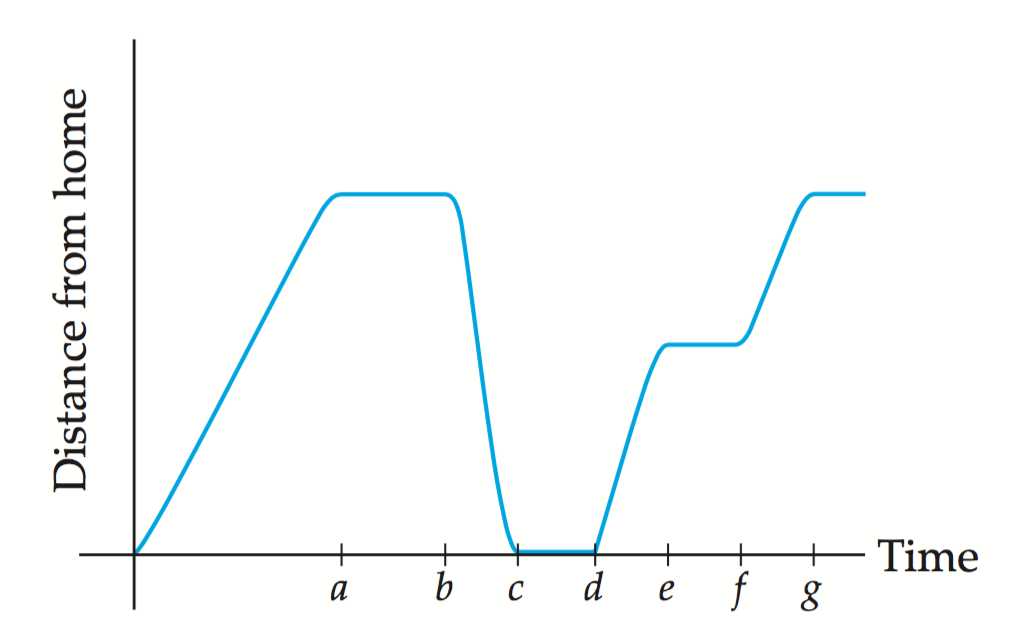
\includegraphics[width=0.7\textwidth]{G9}
\end{center}

\end{frame}

%-----------------------------

\begin{frame}
\frametitle{Edward and Jacob}

Jacob walked at 5 km/h for 20 minutes and then sprinted at 15 km/h for 8 minutes.
\begin{enumerate}
\item How fast would Edward have to walk or run to go the same distance as Jacob did in the same time while moving at a constant speed? 
\item Sketch a graph of Jacob's and Edward's positions over time on the same set of axes.
\end{enumerate}

\end{frame}

%-----------------------------
%  Computations
%-----------------------------
%-----------------------------
%-----------------------------
%-----------------------------
\begin{frame}[t]
\frametitle{A long chain}

The function below has 137 square roots:
	$$
		f(x) = \sqrt{x+ \sqrt{x + \sqrt{x + \sqrt{x+ \ldots + \sqrt{x + \sqrt{x+1}}}}}}
	$$

Find the equation of the line tangent to the graph of $f$ at the point with $x$-coordinate $0$.
\end{frame}

%-----------------------------

\begin{frame}[t]
\frametitle{Computations: Trig derivatives}


Compute the derivatives of the following functions:

\
\begin{enumerate}
%	\item  \DS{f(x) = x \sin x}
	\item  \DS{f(x) = \tan (3x^2+1)}

\vfill
	\item  \DS{f(x) = (\cos x )( \sin 2x )(\tan 3x)}

\vfill
	\item  \DS{f(x) = \cos ( \sin( \tan x))}
\vfill
	\item  \DS{f(x) = \cos \left( 3x + \sqrt{1 + \sin^2 x^2 } \right)}
\vfill
%	\item  \DS{f(x) = \frac{x + \sin x}{x + \cos x}}
\end{enumerate}


\end{frame}

%-----------------------------
%  Differentiation rules
%-----------------------------
%-----------------------------


%-----------------------------
%-----------------------------

\begin{frame}[t]
\frametitle{Vertical things}

\begin{itemize}
	\item Construct a function $f$ that has a \rojo{vertical asymptote} at $x=2$.
	\item Construct a function $g$ that has a \azul{vertical tangent line} at $x=2$.
\end{itemize}

\end{frame}

%-----------------------------


%-----------------------------
\begin{frame}[t]
\frametitle{Absolute value and derivatives - 2}

\begin{block}{True or False?}
For all $n \in \Z$ and all $x$, $\frac{d}{dx}|x|^n=nx|x|^{n-2}$.

\end{block}
\end{frame}

%-----------------------------

%-----------------------------
%  HIGHER ORDER DERIVATIVES
%-----------------------------
%-----------------------------

%-----------------------------
\begin{frame}
\frametitle{Nixon}


Richard Nixon, during the 1972 US Presidential campaign, (paraphrased):

\
\begin{quote}
\emph{Inflation is increasing, but the rate of increase of inflation is decreasing.}
\end{quote}

\vfill

Let 
	\begin{itemize}
		\item $C$ = cost of life
		\item  $t$ = time
	\end{itemize}
What did Nixon say in terms of derivatives?

\vfill

\end{frame}
%-----------------------------
%  CHAIN RULE
%-----------------------------
%------------------------------

\begin{frame}
\frametitle{Chain rule from a graph}


If $f$ and $g$ are the functions whose graphs are shown. \\
Let $u(x)=f(g(x))$ and $v(x)=g(f(x))$. \\ \medskip

Find each derivative, if it exists. \\ If it does not exist, explain why.


\begin{enumerate}
\item $u'(1)$
\item $v'(1)$
\end{enumerate}
\vspace{-1cm}


\begin{center}
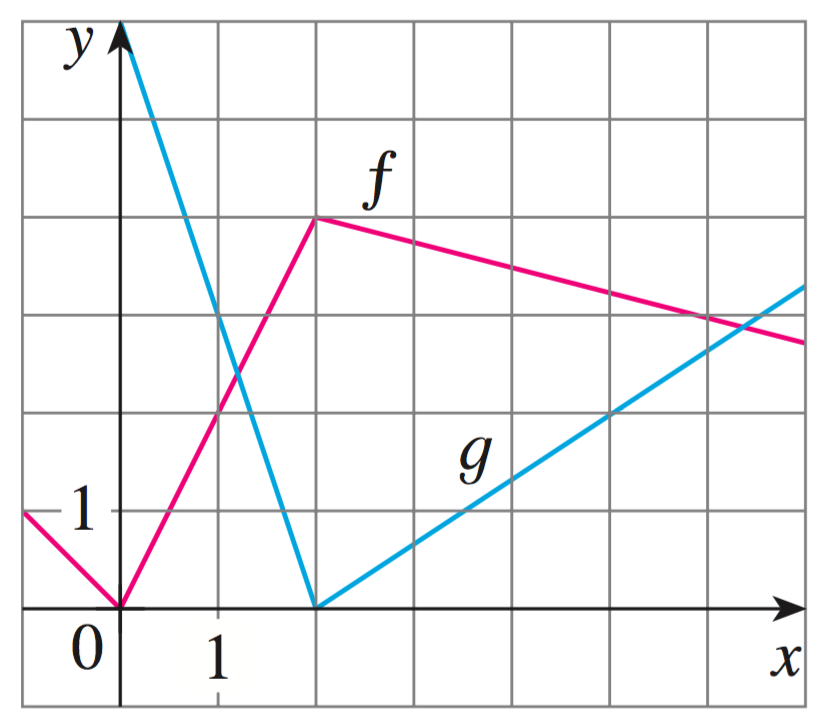
\includegraphics[width=0.5\textwidth]{G10}
\end{center}

\end{frame}

%-----------------------------

\begin{frame}[t]
\frametitle{Balloon}

I am inflating a spherical balloon.  Below is the graph of the radius $r$ (in $cm$) as a function of time $t$ (in $s$).
 At what rate is the volume of the balloon increasing at time $4s$?

\begin{center}
	\only<1>{
		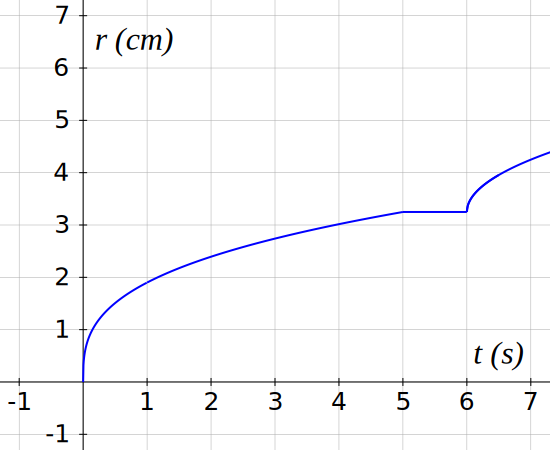
\includegraphics[scale=.35]{G6}
		}
	\only<2>{
		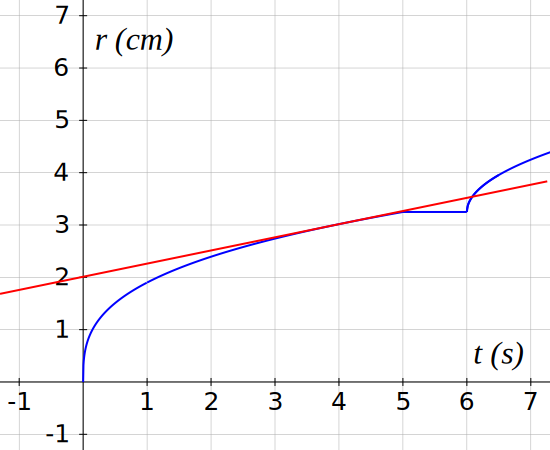
\includegraphics[scale=.35]{G7}
		}
\end{center}

\end{frame}
%-----------------------------

\begin{frame}[t]
\frametitle{An alternative proof of the quotient rule}

Assume we have already proven the product rule, the power rule, and the chain rule.

Obtain a formula for the derivative of \DS{h(x) = \frac{f(x)}{g(x)}}.

\emph{Hint:}  \DS{\frac{f(x)}{g(x)} = f(x) \cdot g(x)^{-1}}

\end{frame}

%-----------------------------

\begin{frame}
\frametitle{Derivatives of \DS{(f \circ g)}}

Assume $f$ and $g$ are functions that have all their derivatives. 
 Find formulas for
	\begin{enumerate}
		\item  \DS{(f \circ g)'(x)}
		\item  \DS{(f \circ g)''(x)}
		\item	\DS{(f \circ g)'''(x)}
	\end{enumerate}
	
	in terms of the values of $f$, $g$ and their derivatives.
	
	\
	
	\emph{Hint:}  The first one is simply the chain rule.
	
	\ \p
	
	\emph{Challenge:} Find a formula for \DS{(f \circ g)^{(n)}(x)} \\
	(This is beyond the scope of this course).  
\end{frame}

%-----------------------------
%  TRIG
%-----------------------------
%-----------------------------

\begin{frame}[t]
\frametitle{Derivative of $\cos$}


Let \DS{g(x) = \cos x.}

\

Obtain and prove a formula for its derivative directly from the definition of derivative as a limit.

\vfill


{\bf Hint:}  Imitate the derivation in Video 3.12. \\  If you need a trig identity that you do not know, google it or ask another student.

%{\bf Hint:}  This identity may come in handy:
%	$$
%		\cos (a + b) = \cos a \cos b - \sin a \sin b
%	$$
\end{frame}

%-----------------------------
\begin{frame}[t]
\frametitle{Derivatives of the other trig functions}


Use the basic differentiation rules, as well as
	$$
		\frac{d}{dx} \sin x = \cos x, \quad \quad \frac{d}{dx} \cos x = - \sin x,
	$$
to quickly obtain and prove formulas for the derivatives of $\tan$, $\cot$, $\sec$, and $\csc$.

\end{frame}

%-----------------------------


\begin{frame}
\frametitle{Product of trig functions}

Let $f(x)= \sin x \cos x$.  What is its derivative $f'(x)$?
\begin{enumerate}
\item $1-2\sin^2(x)$
\item $2\cos^2(x) -1$
\item $\cos 2x$
\item all of the above
\item none of the above
\end{enumerate}

%Answer: (d).} (a) - (c) are equivalent formulae. One can get (a) by using the product rule and $\cos^2(x)=1-\sin ^2(x)$.
\end{frame}

%-----------------------------

\begin{frame}[t]
\frametitle{A pesky function}

Let \DS{h(x) = \begin{cases} x^2 \sin \dfrac{\;1\;}{x} & \mbox{ if } x \neq 0 \\ 0 & \mbox{ if } x=0 \end{cases}}.

	\begin{enumerate}
		\item  Calculate \DS{h'(x)} for any $x \neq 0$.
		\item  \label{it:0a} Using the definition of derivative, calculate \DS{h'(0)}.
		\item \label{it:0b}  Calculate \DS{\lim_{x \to 0} h'(x)}
		
		\vspace{.2cm}
		{\smallerfont \emph{Hint:} Questions \ref{it:0a} and \ref{it:0b} have different answers.}
		
		\p \vspace{.2cm}
		\item  Is $h$ continuous at $0$?
		\item Is $h$ differentiable at $0$?
		\item  Is $h'$ continuous at $0$?
	\end{enumerate}

\end{frame}
%-----------------------------
%  IMPLICIT DIFFERENTIATION
%-----------------------------
%-----------------------------

\begin{frame}[t]
\frametitle{Implicit differentiation}

The equation
	$$
		\sin (x+y) + xy^2 = 0
	$$
defines a function \DS{y=h(x)} near $(0,0)$.
\href{https://www.desmos.com/calculator/bvupq00r6s}{\beamergotobutton{graph}}


Using implicit differentiation, compute
	\begin{multicols}{4}
	\begin{enumerate}
		\item \DS{h(0)}
		\item \DS{h'(0)}
		\item \DS{h''(0)}
		\item \DS{h'''(0)}
	\end{enumerate}
	\end{multicols}
\end{frame}

%------------------------------
%-----------------------------
\end{document}
%-----------------------------
%-----------------------------









